\section{Theorie}
\label{sec:theorie}
\textbf{Grundlagen der Voltammetrie un der Elektrochemischen Spannungsreihe!}\\
\subsection{Voltammetrie}
Voltammetrie ist eine Sammelbezeichnung für einige elektrochemische Analysemethoden, bei denen die Spannung (das Potential) und der fließende Strom zwischen mindestens zwei Elektroden betrachtet werden, um daraus Aussagen zur Zusammensetzung einer Probe abzuleiten.\\
Die \textit{Voltammetrie} ist nicht mit der \textit{Voltametrie} zu verwechseln. Bei letzterer wird lediglich die Spannung gemessen.
\subsection{Die Elektrochemische Spannungsreihe}


Die Elektrochemische Spannungsreihe ordnet Metalle nach ihrem elektrochemischen Potential. Als Bezug dient dabei stets die Standardwasserstoffelektrode. In Verbindung letzterer Halbzelle mit einem Metall, in seiner einmolaren Metallsalzlösung bei Standardbedingungen, kann das Standardpotential des Metalls als anliegende Spannung zwischen den Elektroden gemessen werden. Das Vorzeichen der Standardpotentiale sagt aus, in welche die Richtung Elektronen strömen. Es besteht ein direkter Zusammenhang zwischen dem Standardelektrodenpotential eines Metalls und dessen Bestreben reduziert zu werden. Je größer das Elektrodenpotential ist, umso edler ist auch das Metall und umso eher wird es reduziert. Verwendung findet dieser Umstand zum Beispiel in der Berechnung galvanischer Elemente. Im folgenden kann anhand der Standardelektrodenpotentiale gelöster Metallionen deren Positionierung in einem Polarogramm abgeleitet werden.\cite{spannungsreihe}\\

\vline

\subsection{Analyse der Polarogramme}
Grundlage für die Analyse der enthaltenen Metall-Ionen ist die aufgenommene Strom-Spannungs-Kurve des Polarographen. Aufgrund der spezifischen Halbstufenpotentiale von Metall-Ionen ändert sich bei unterschiedlichen Arbeitspotentialen die gemessene Stromstärke. Dieser Strom an der Arbeitselektrode 
tritt als Folge der Reduktionsreaktion der Metall-Ionen auf und ist direkt proportional zur Konzentration des umgesetzten Stoffes. Der Strom im Zusammenhang mit diesem Massentransport der Ionen wird als \textsc{Faraday}scher Strom bezeichnet. \linebreak Um eine ausreichende Leitfähigkeit und somit einen entsprechenden Ladungstransport in der Lösung garantieren zu können, werden den untersuchten Proben oft Grundelektrolyten in Form von Salzen, Säuren oder Basen zugegeben.\linebreak
Aufgrund der spezifischen Halbstufenpotentiale lassen sich qualitative Ergebnisse dieses Verfahrens auswerten. Betrachtet man jedoch auch den Zusammenhang des Stromflusses bei einem bestimmten Arbeitspotential mit der Konzentration des umgesetzten Stoffes, so lassen sich ebenfalls quantitative Bewertungen äußern.\linebreak
Für diese Betrachtung ist jedoch eine Form der Kalibrierung notwendig, um die gemessenen Signale quantitativ auswerten zu können. Dies ist zum einen über einen externen oder internen Standard möglich, jedoch wurde sich aufgrund der geringen zu bestimmenden Konzentrationen in diesem Versuch für die Aufstockmethode, auch Standardadditionsmethode genannt, entschieden. Möchte man einen internen oder externen Standard nutzen so sind in diesem Fall ebenfalls Kalibrierkurven mit linearem Zusammenhang mittels bekannter Referenz aufzustellen.\linebreak
Bei dieser Methode wird in diesem Versuch nach der polarographischen Analyse der unbehandelten Probe, eine definierte Menge eines bekannten Standards zugegeben. Dieser Standard enthält dabei den zu bestimmenden Stoff in einer exakt bekannten Konzentration. Aus den gemessenen Datenpunkten lässt sich nun eine Geradengleichung bestimmen (siehe Abb. \ref{fig:standardaddition} und Gl. \ref{gl:1}).

\begin{flalign}
\label{gl:1}
Y &= \frac{\Delta y}{\Delta x}*X+yA
\end{flalign}

%Start
\begin{figure}[h!]
	\centering
	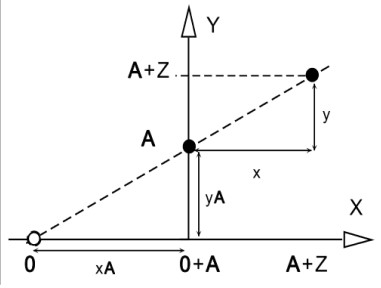
\includegraphics[width=0.5\textwidth]{img/Standardaddition}
	\caption{Darstellung der Standardadditionsmethode \cite{}}
	\label{fig:standardaddition}
\end{figure}
\FloatBarrier
%Ende

Aus der ermittelten Geradengleichung, lässt sich nun, aufgrund der geometrischen Beziehung der Strahlensätze, die Konzentration der Probe über den Wert $xA$ in Abb. \ref{fig:standardaddition} bestimmen. Eine Herleitung dazu ist unter Gl. \ref{gl:2} und Gl. \ref{gl:3} zu finden. Die Bedeutungen der Variablen sind nachfolgend in der Tabelle \ref{tab:variablen} aufgeführt.

\begin{flalign}
\label{gl:2}
	Y &= \frac{y}{x}*X+yA\\
	X&= \frac{Y-yA}{\frac{y}{x}}
\end{flalign}

\textit{Für $Y=0$ heißt das:}

\begin{flalign}
\label{gl:3}
X&= xA = \frac{0-yA}{\frac{y}{x}} = \frac{-yA}{\frac{y}{x}}\\
xA&= -c\\
c	&= \underline{\underline{\frac{yA}{\frac{y}{x}}}}
\end{flalign}

\vspace*{-5mm}

%Tabelle START
\renewcommand{\arraystretch}{1.2}
\begin{table}[h!]
	\centering
	%\caption{Variablen der Abb.\ref{fig:standardaddition} und der Tab.\ref{tab:variablen} und ihre Bedeutungen}
	\caption{Variablen und ihre Bedeutung}
	\label{tab:variablen}
	%\makebox[\textwidth]{
	%	\resizebox{17cm}{!}{
			\begin{tabular}{c|c}
				\hline
				\textbf{Variable}&\textbf{Bedeutung} \\
				\hline
				A& Analyt \\
				Z& Zugabe\\
				$Y$& Signalwert\\
				$yA$& Signalwert der Testlösung - nur Analyt\\
				$\Delta y$& Signaländerungnach Zugabe der Standardlösung \\
				$X$& Anylytwert\\
				$xA$&Analytkonzentration in der Testlösung\\
				$\Delta x$& Konzentrationsändeung durch Standard-Zugabe \\
				\hline	
			\end{tabular}
		%	}
			%}
		\end{table}
		\FloatBarrier
		\vspace*{-2.5mm}
		%Tabelle Ende

